%=================================================================

\section{Introduction}\label{sec-intro}


%\todo{Narrow down to a topic; Dig a hole; Fill the hole}




%\gangli{``narrow in on topic'' reminds you 
%that readers and reviewers only know that this is a AI or HTM research paper (and maybe have read the title/abstract). 
%You need to help them figure out what topic and area of research paper this is. 
%You _don't_ need to wax poetic about the topic's importance.}

%\gangli{`dig a hole'' reminds you that 
%you need to convince the reader that there's a problem with the state of the world. 
%Prior work may exist but it's either missing something important or there's a missing opportunity. 
%The reader should be drooling for a bright future just out of reach.}

%\gangli{``fill the hole'' reminds you to show the reader 
%how and why the paper they're reading will fix these problems and deliver us into a better place. 
%You don't need a whirlwind summary of the technical details, 
%but you need readers convinced (and in a good mood) to keep reading.}





%\todo{The importance of the area}
%\blindtext

Credit card fraud identification is an important financial risk management task aimed at detecting possible fraud in credit card transactions. With the popularity of electronic payments, credit card fraud has become a serious problem in the global financial business. Fraud may include skimming, stolen credit cards, fraudulent transactions, and other fraudulent tactics.

The core of this task is to analyze and model large amounts of credit card transaction data by using machine learning and data mining techniques in order to identify potential frauds.


%\todo{The problems faced by most current methods}
%\blindtext

The data processed in this paper contains transaction times, amounts, and 28 preprocessed features.In this paper, anomaly detection will be investigated on this dataset using four different algorithms incorporating unsupervised learning and supervised learning.

%\todo{What can be addressed by existing methods; Why those problems are challenges to existing methods?}
%\blindtext
\section{Data Analysis and Preprocessing} \label{sec-preliminaries}
The time field in the dataset of this paper represents the time of the transaction converted to seconds during the day. In addition to the 28 processed features, the categories of real transaction amount and altered behavior are also included.Category 0 indicates normal and category 1 indicates abnormal.
The dataset contains 284807 behavioral data, of which there are 284315 normal behaviors and 492 abnormal behaviors.This dataset is a typical unbalanced dataset for anomaly detection task.

By plotting scatter plots about time and transaction amount we find that the anomalous behavior is more evenly distributed over time and the anomalous behavior has a lower transaction amount, so we include both features in our analysis.
\begin{figure}[H]
  \centering
\selectcolormodel{rgb}
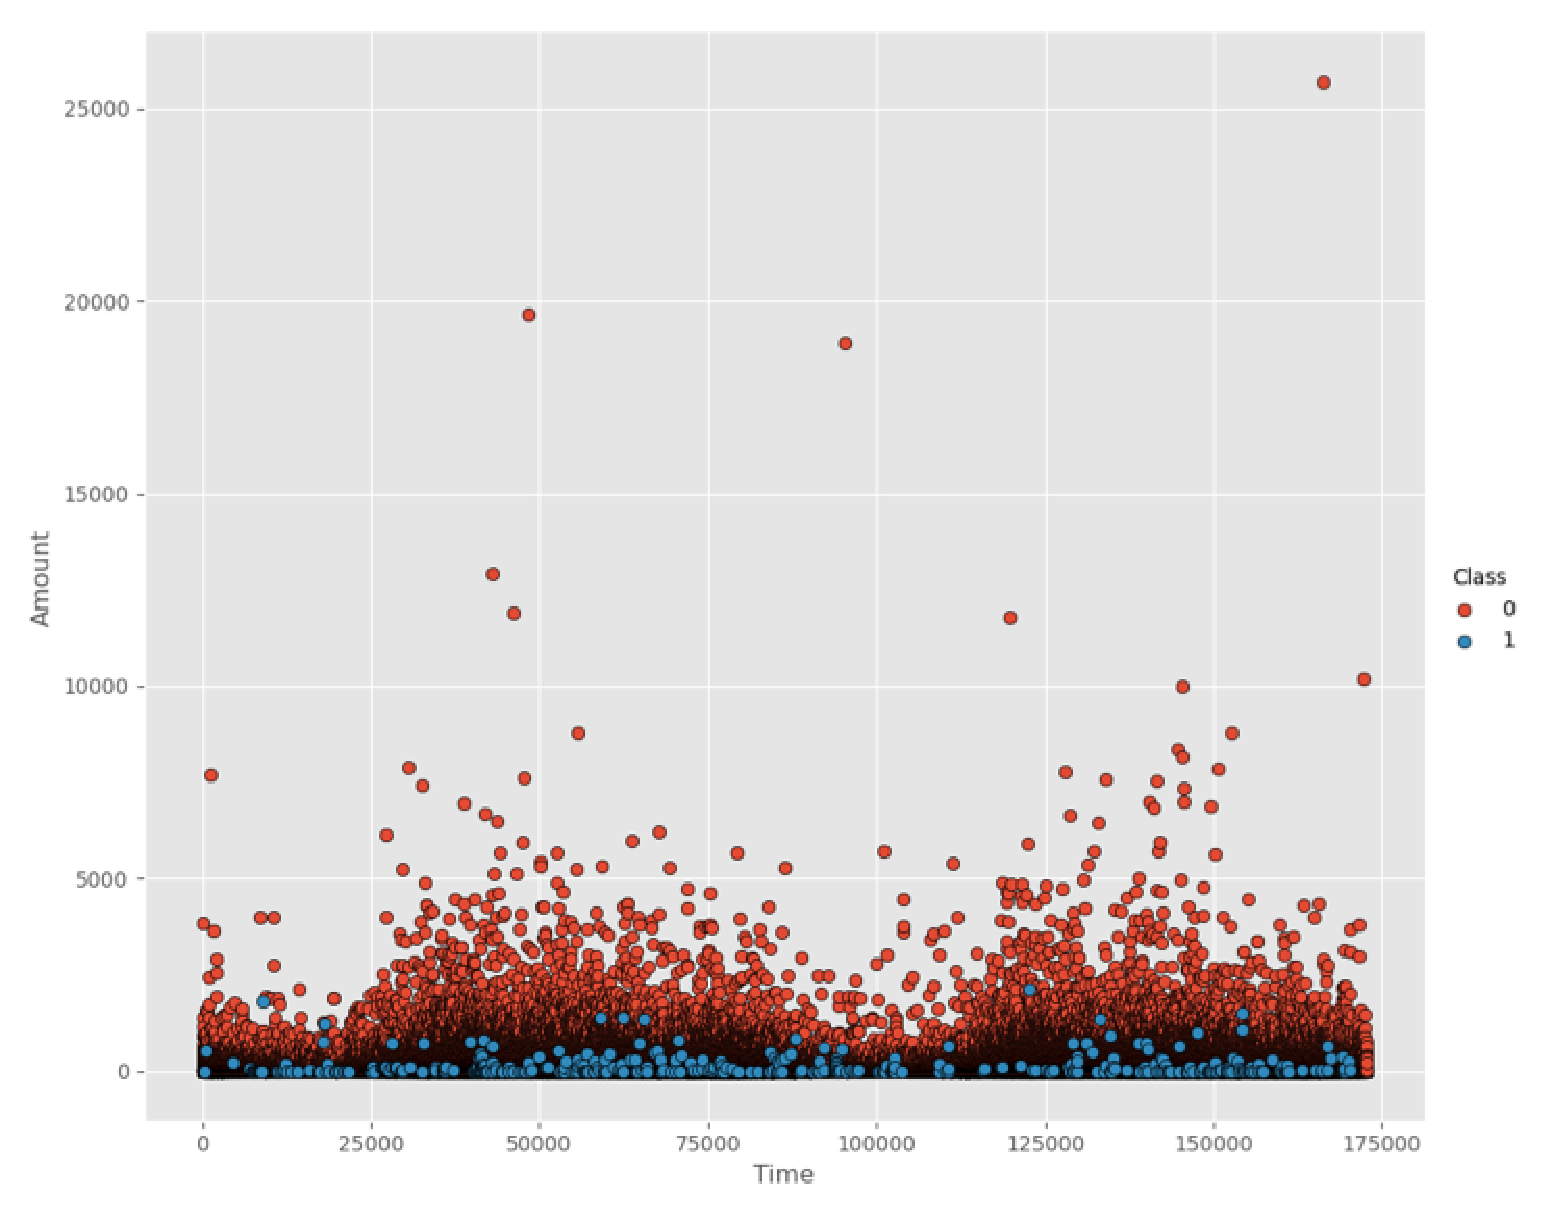
\includegraphics[scale=0.45]{amounttime.eps}
%  \includegraphics[width=0.5\textwidth]{figures//OutAspect_target.eps}\\
\caption{Amount and Time Distribution Scatterplot}\label{fig:OutAspect-target}
\end{figure}
Meanwhile, this paper also analyzes the direct correlation between features and characteristics, and features and categories. By analyzing the correlation matrix we found that V17, V14, V12, and V10 are negatively correlated with aberrant behavior, and V2, V4, V11, and V19 are positively correlated with aberrant behavior. Most of the features are not correlated with each other.
\begin{figure}[H]
	\centering
	\selectcolormodel{rgb}
	\includegraphics[scale=0.23]{correlation.eps}
	%  \includegraphics[width=0.5\textwidth]{figures//OutAspect_target.eps}\\
	\caption{Correlation Matrices}\label{fig:OutAspect-target}
\end{figure}
In this paper, the vector distribution of data points is also explored, and a two-dimensional scatter plot is drawn by PCA and t-SNE dimensionality reduction. As can be seen from the t-SNE plot, the anomalies are clustered and relatively independent of the normal points.

\begin{figure}[H]
	\centering
	\selectcolormodel{rgb}
	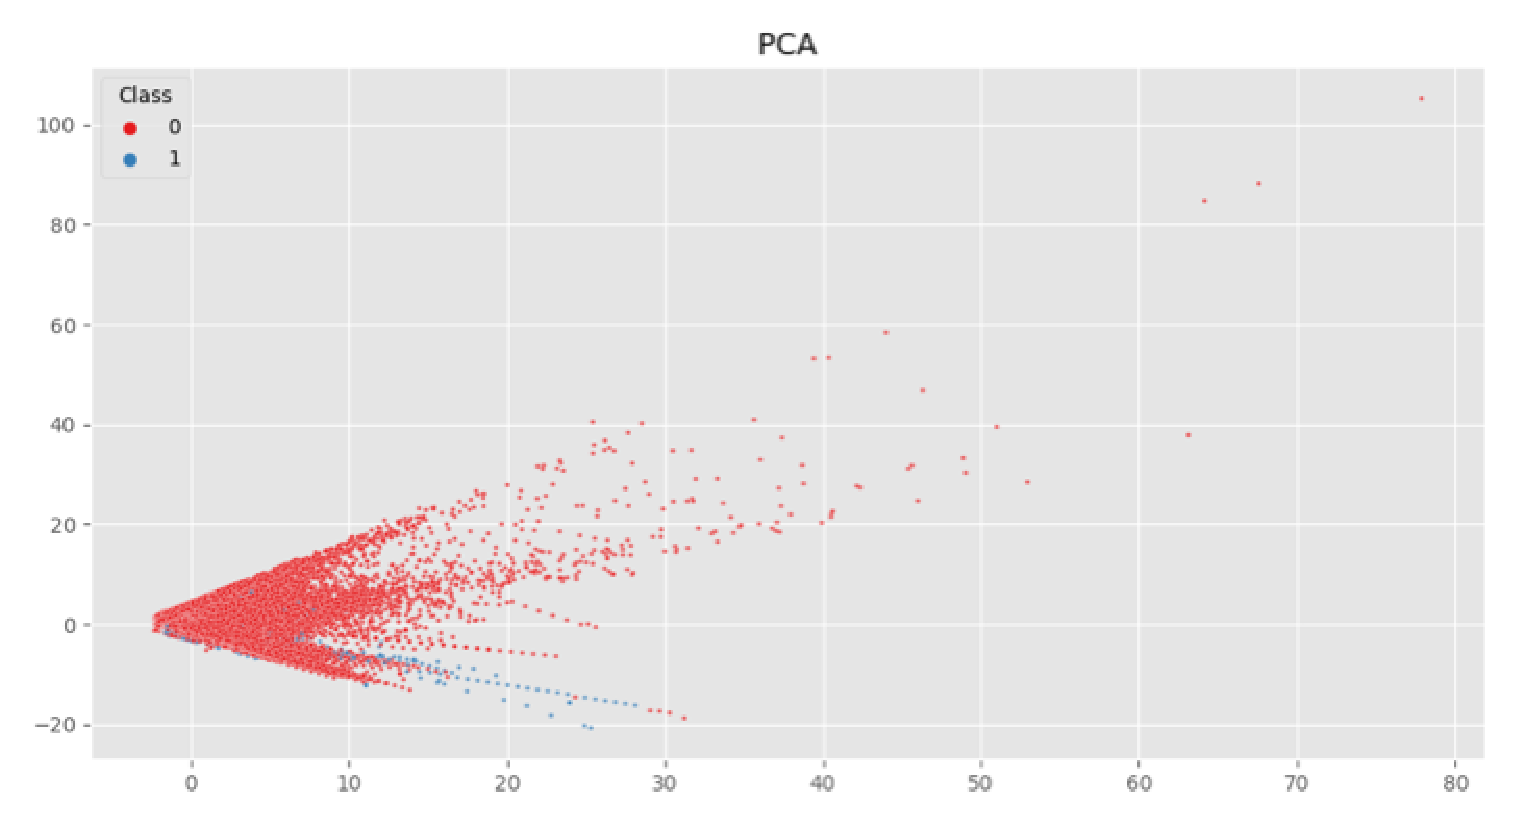
\includegraphics[scale=0.4]{pca.eps}
	%  \includegraphics[width=0.5\textwidth]{figures//OutAspect_target.eps}\\
	\caption{PCA}\label{fig:OutAspect-target}
\end{figure}
\begin{figure}[H]
	\centering
			\selectcolormodel{rgb}
	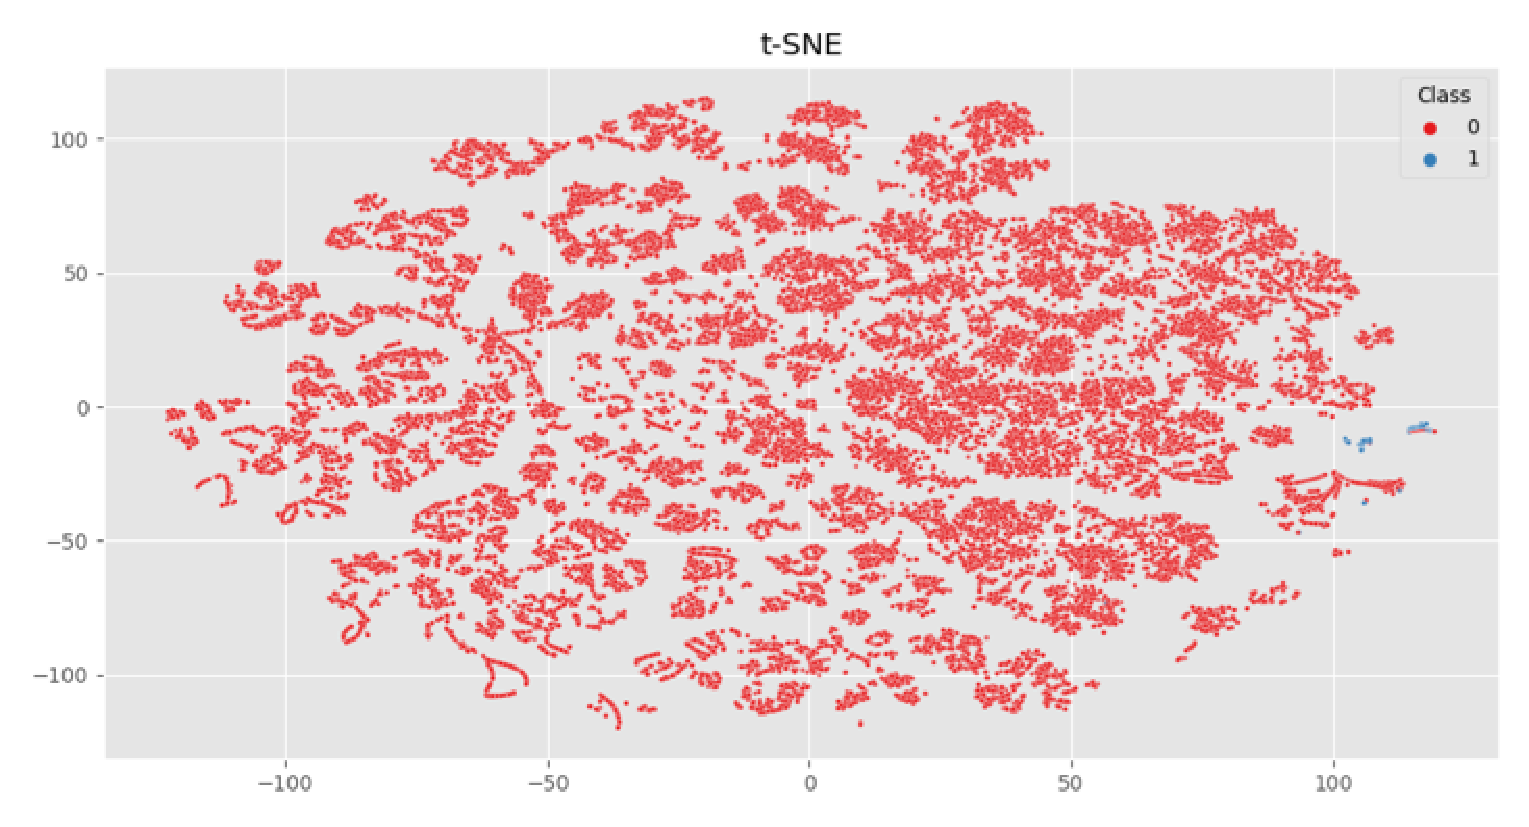
\includegraphics[scale=0.4]{tsne.eps}
	%  \includegraphics[width=0.5\textwidth]{figures//OutAspect_target.eps}\\
	\caption{t-SNE}\label{fig:OutAspect-target}
	\end{figure}
For the model training, this paper preprocesses the data, normalizing and normalizing Time and Amount. At the same time, the training set and test set are divided to facilitate the training of supervised learning models.The training set is 80\% and the test set is 20\%.30 selected features are  [’Time’,’Amount’,’V1’, ’V2’, ’V3’, ’V4’, ’V5’, ’V6’, ’V7’, ’V8’, ’V9’, ’V10’,’V11’,’V12’, ’V13’, ’V14’, ’V15’, ’V16’, ’V17’, ’V18’, ’V19’, ’V20’, ’V21’, ’V22’, ’V23’, ’V24’,’V25’, ’V26’, ’V27’, ’V28’].
\begin{center}
	\begin{tabular}{c| c c c c c }
		\toprule
		%\centering
		Data & \texttt{row_num}  & \texttt{Normal} & \texttt{Fraud} \\
		\midrule
		$train$
		&  {$227845$} &  {$227468$} &  {$377$} \\
		$test$
		&  {$57339$} &  {$56847$} &  {$115$} \\
		\bottomrule
	\end{tabular}
\end{center}

\section{Unsupervised and Supervised Anomaly Detection Methods} \label{sec-method}
In this paper, two unsupervised and two supervised anomaly detection algorithms will be presented, they are Isolation Forest, DBSCAN Clustering, Random Forest and XGBoost.
Isolation Forest(IF) is build based on decision trees. No pre-defined labels here. An
unsupervised learning algorithm.

1. Two quantitative properties of anomalous data points:Outliers are few and their
features are very different from normal points.

2. Not assume normal distribution and Detect outliers at a multi-dimensional level.

3. Isolation Forest is computationally efficient: a low constant and a low memory
requirement.

4.Main Parameters - Number of estimators, Max samples, Contamination, Max features
	\begin{figure}[H]
	\centering
\selectcolormodel{rgb}
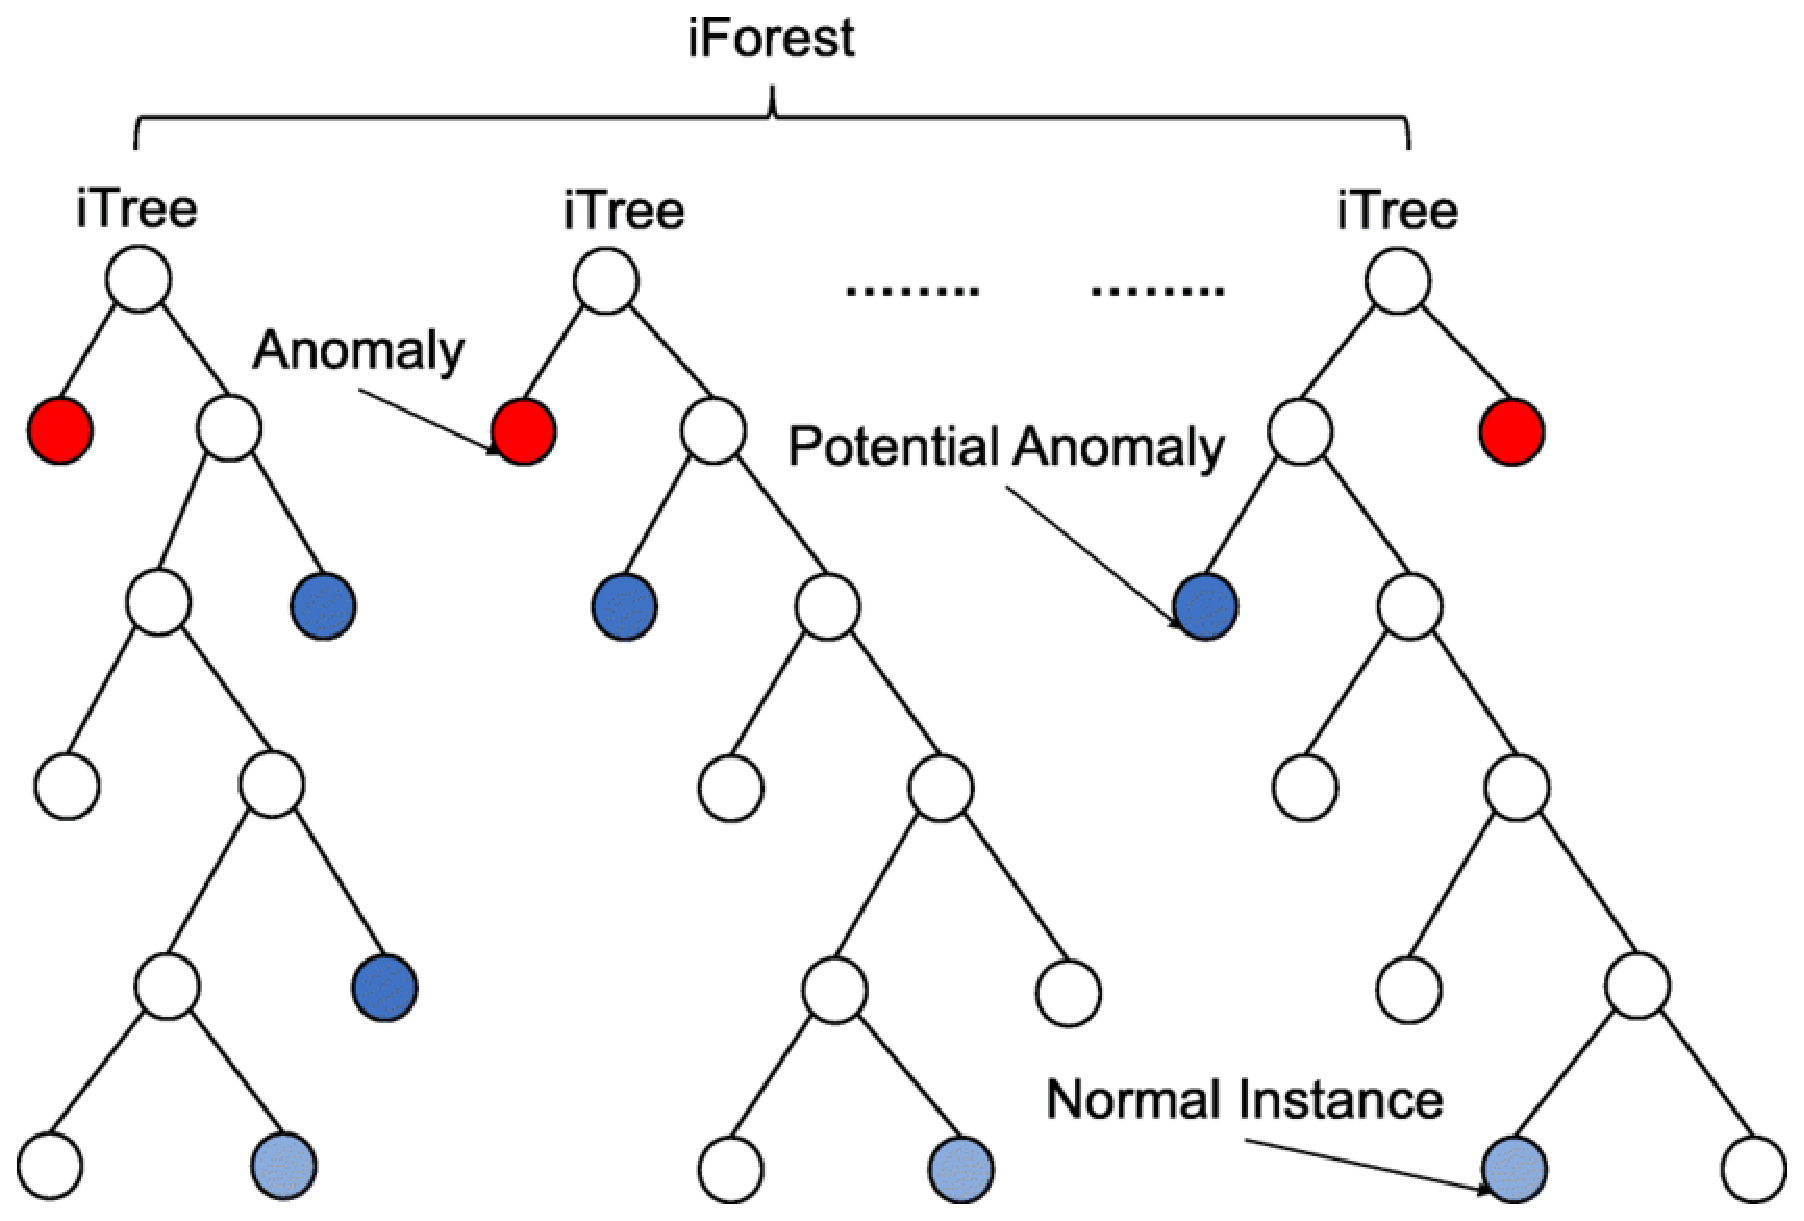
\includegraphics[scale=0.2]{iforest.eps}
%  \includegraphics[width=0.5\textwidth]{figures//OutAspect_target.eps}\\
% \caption{Aggregated time series}\label{fig:OutAspect-target}
\end{figure}
DBSCAN is a powerful density-based data clustering algorithm.

1. DBSCAN algorithm separates the high-density regions of the data from the low-density areas.

2. Detect outliers by identifying noise.

3. Main Parameters - Epsilon, minPoints
	\begin{figure}[H]
	\centering
\selectcolormodel{rgb}
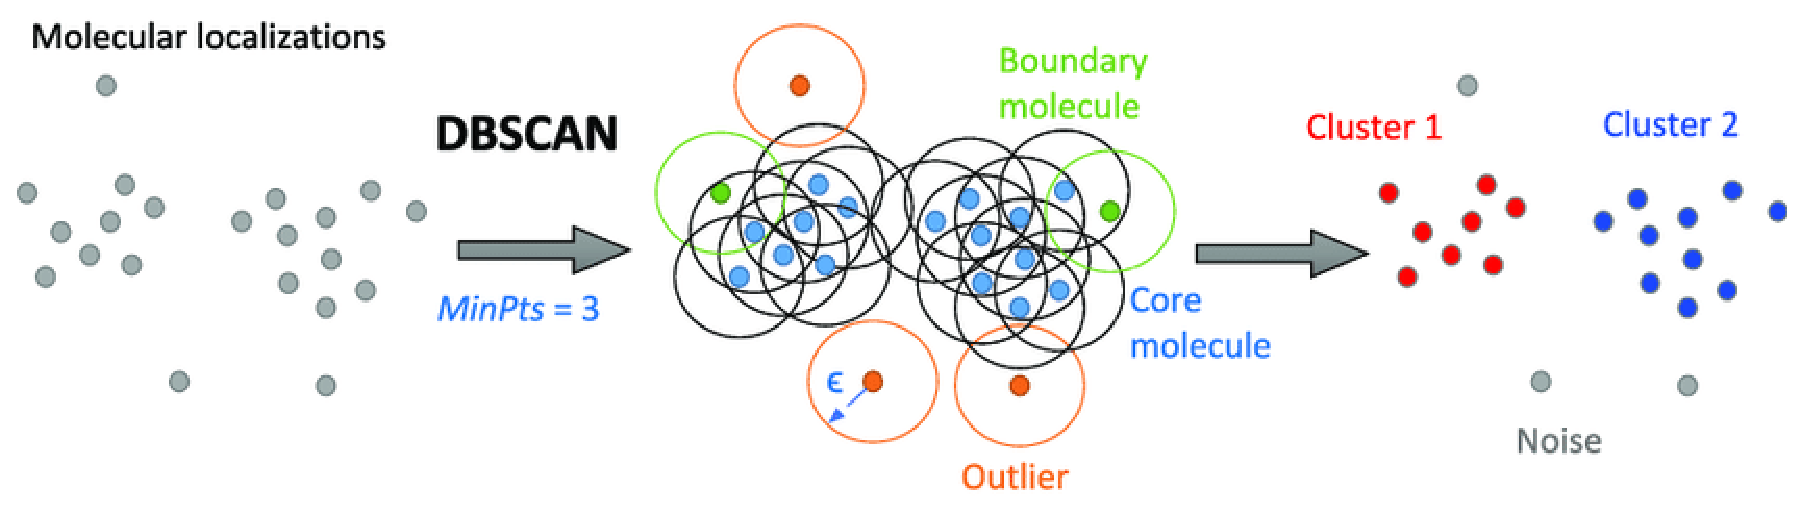
\includegraphics[scale=0.4]{dbscan.eps}
%  \includegraphics[width=0.5\textwidth]{figures//OutAspect_target.eps}\\
% \caption{Aggregated time series}\label{fig:OutAspect-target}
\end{figure}
Random Forests perform classification by constructing multiple decision trees and combining their predictions.

1. Constructing a decision tree from the train set.

2. Prediction of test sets and feature importance exploration

3. Main Parameters - n\_estimators, max\_depth, min\_samples\_leaf,min\_samples\_split
	\begin{figure}[H]
	\centering
	\selectcolormodel{rgb}
	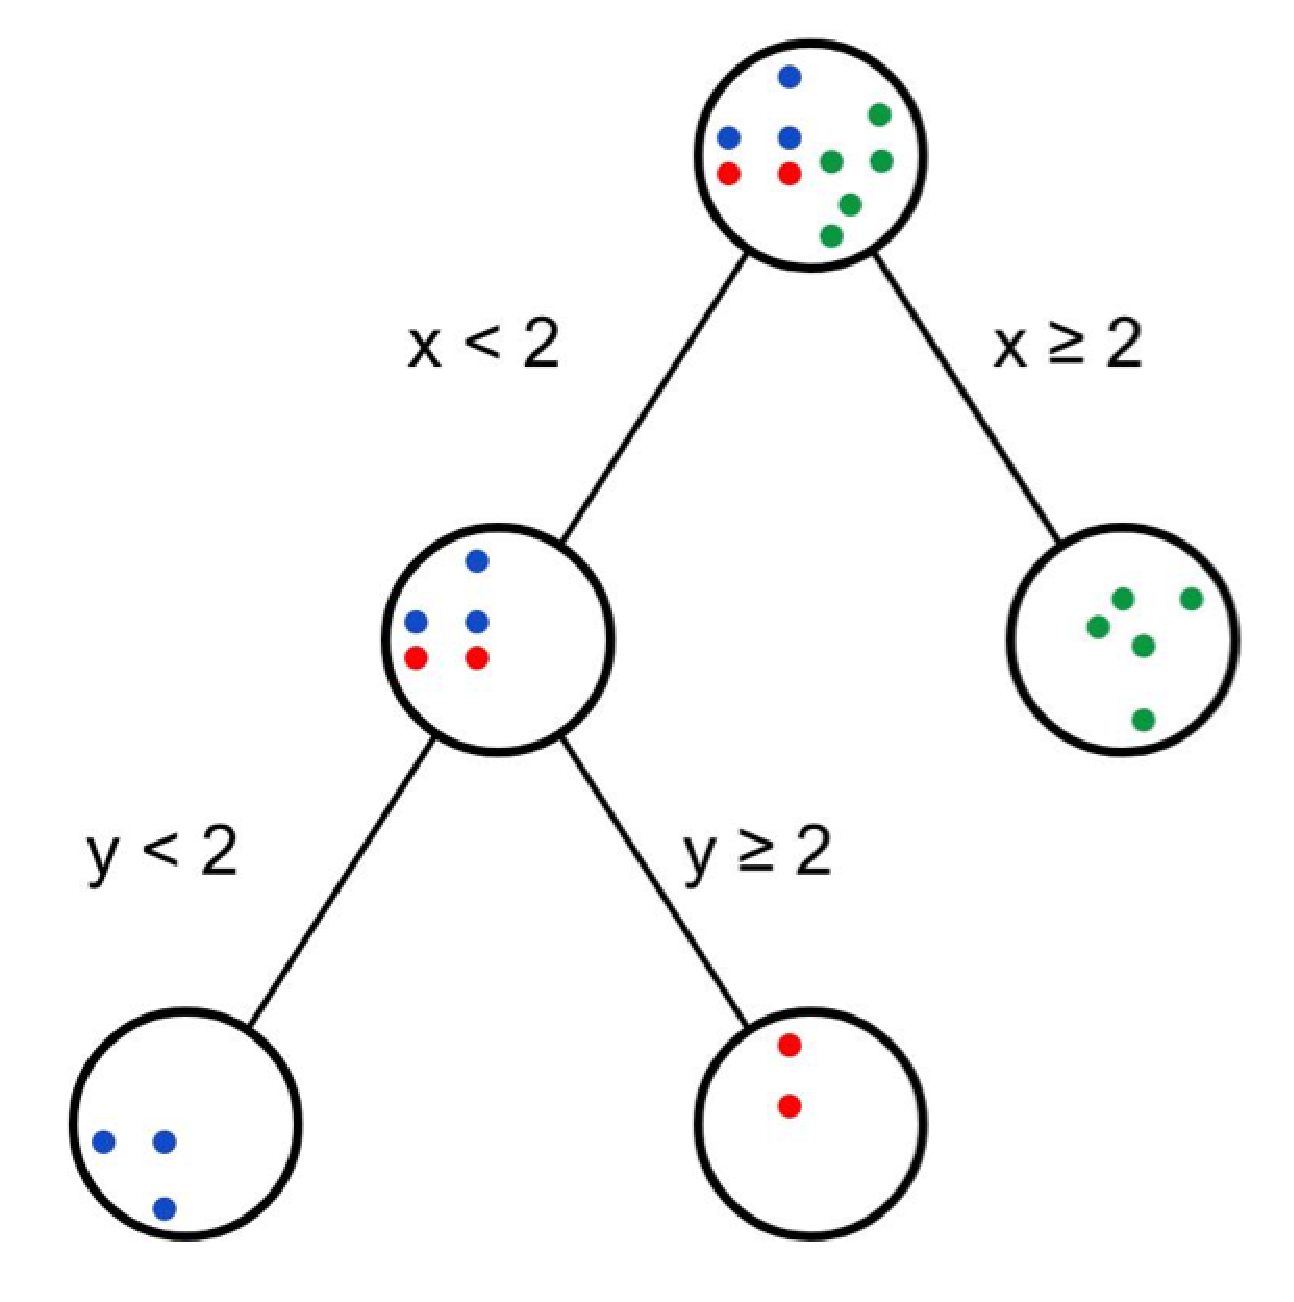
\includegraphics[scale=0.3]{rf.eps}
	%  \includegraphics[width=0.5\textwidth]{figures//OutAspect_target.eps}\\
	% \caption{Aggregated time series}\label{fig:OutAspect-target}
\end{figure}
XGBoost (eXtreme Gradient Boosting) is a gradient boosting tree algorithm.

1. The core principle is to combine multiple weak learners (decision trees) into one
strong learner

2. Decision trees are trained in an iterative manner to train new trees based on the
residuals between the predictions and the actual labels of all the previous trees in
order to gradually reduce the error.

3. Main Parameters - n\_estimators, max\_depth, learning\_rate, subsample,
colsample\_bytree
	\begin{figure}[H]
	\centering
	\selectcolormodel{rgb}
	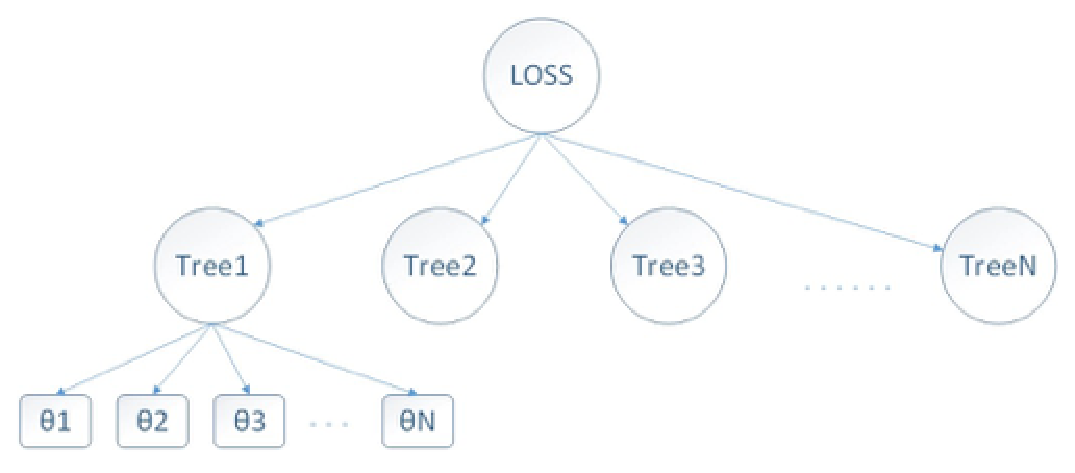
\includegraphics[scale=0.5]{xgb.eps}
	%  \includegraphics[width=0.5\textwidth]{figures//OutAspect_target.eps}\\
	% \caption{Aggregated time series}\label{fig:OutAspect-target}
\end{figure}
\section{Model Train and Result} \label{sec-experiment}
In this paper, we perform parameter tuning for all four models mentioned above, for unsupervised model we use full data for training and prediction, for supervised model we use training set and test separately for training and prediction. The model parameters are shown in the following table.

\begin{center}
	\begin{tabular}{c| c c c c c }
		\toprule
		%\centering
		Method & \texttt{Type}  & \texttt{Train} & \texttt{Test}  \\
		\midrule
		$Isolation\ Forest$
		&  {$Unsupervised$} &  {$all\ data$} & {$all\ data$} \\
		$DBSCAN$
		&  {$Unsupervised$} &  {$all\ data$} & {$all\ data$} \\
		$Random\ Forest$
		&  {$Supervised$} &  {$train$} &  {$test$}  \\
		$XGBoost$
		&  {$Supervised$} &  {$train$} &  {$test$}  \\
		\bottomrule
	\end{tabular}
\end{center}
\begin{center}
	\begin{tabular}{c| c c c c c }
		\toprule
		%\centering
		Method & \texttt{ Parameters} \\
		\midrule
		$Isolation\ Forest$
		&   {$n\_estimators=1000,contamination=0.00172,max_features=1.0$} \\
		$DBSCAN$
		&  {$eps=3.0, min\_samples=10$} \\
		$Random\ Forest$
		&  {$n\_estimators=100$} \\
		$XGBoost$
		&  {$n\_estimators=100,learning\_rate=0.3,max\_depth=5$} \\
		\bottomrule
	\end{tabular}
\end{center}
In this paper, the commonly used accuracy, accuracy, recall, and F1 values are used to evaluate the model. As shown in the following formula, where TP stands for True Fraud, TN for True Normal, FP for False Normal, and FN for False Fraud.
	\begin{align}
	\text{Accuracy} = \frac{TP + TN}{TP + TN + FP + FN}
\end{align}
\begin{align}
	\text{Precision} = \frac{TP}{TP + FP}
\end{align}
\begin{align}
	\text{Recall} = \frac{TP}{TP + FN}
\end{align}
\begin{align}
	\text{F1-score} = 2 \times \frac{\text{Precision} \times \text{Recall}}{\text{Precision} + \text{Recall}}
\end{align}
The final evaluation metrics for each model are shown in the table below. Among them, the overall indexes of unsupervised models are not as good as supervised models, and DBSCAN has the worst recognition results, while the two supervised models are based on decision trees, and there is not much difference in the indexes, and the difference is that XGBoost has a shorter running time. In summary, for task data among the four models, XGBoost can accurately identify most of the abnormal behaviors and has a shorter running time for better performance.
\begin{center}
	\begin{tabular}{c| c c c c c }
		\toprule
		%\centering
		Method & \texttt{Accuracy}  & \texttt{Precision} & \texttt{Recall}  & \texttt{F1}  & \texttt{Time(s)}\\
		\midrule
		$Isolation\ Forest$
		&  {$0.998$} &  {$0.314$} & {$0.313$} & {$0.314$}  & {$344$} \\
		$DBSCAN$
		&  {$0.946$} &  {$0.027$} & {$0.865$} & {$0.053$}  & {$182$} \\
		$Random\ Forest$
		&  {$0.999$} &  {$0.948$} & {$0.791$} & {$0.863$}  & {$314$} \\
		$XGBoost$
		&  {$0.999$} &  {$0.949$} & {$0.817$} & {$0.874$}  & {$56$} \\
		\bottomrule
	\end{tabular}
\end{center}

	\begin{figure}[H]
	\centering
		\selectcolormodel{rgb}
	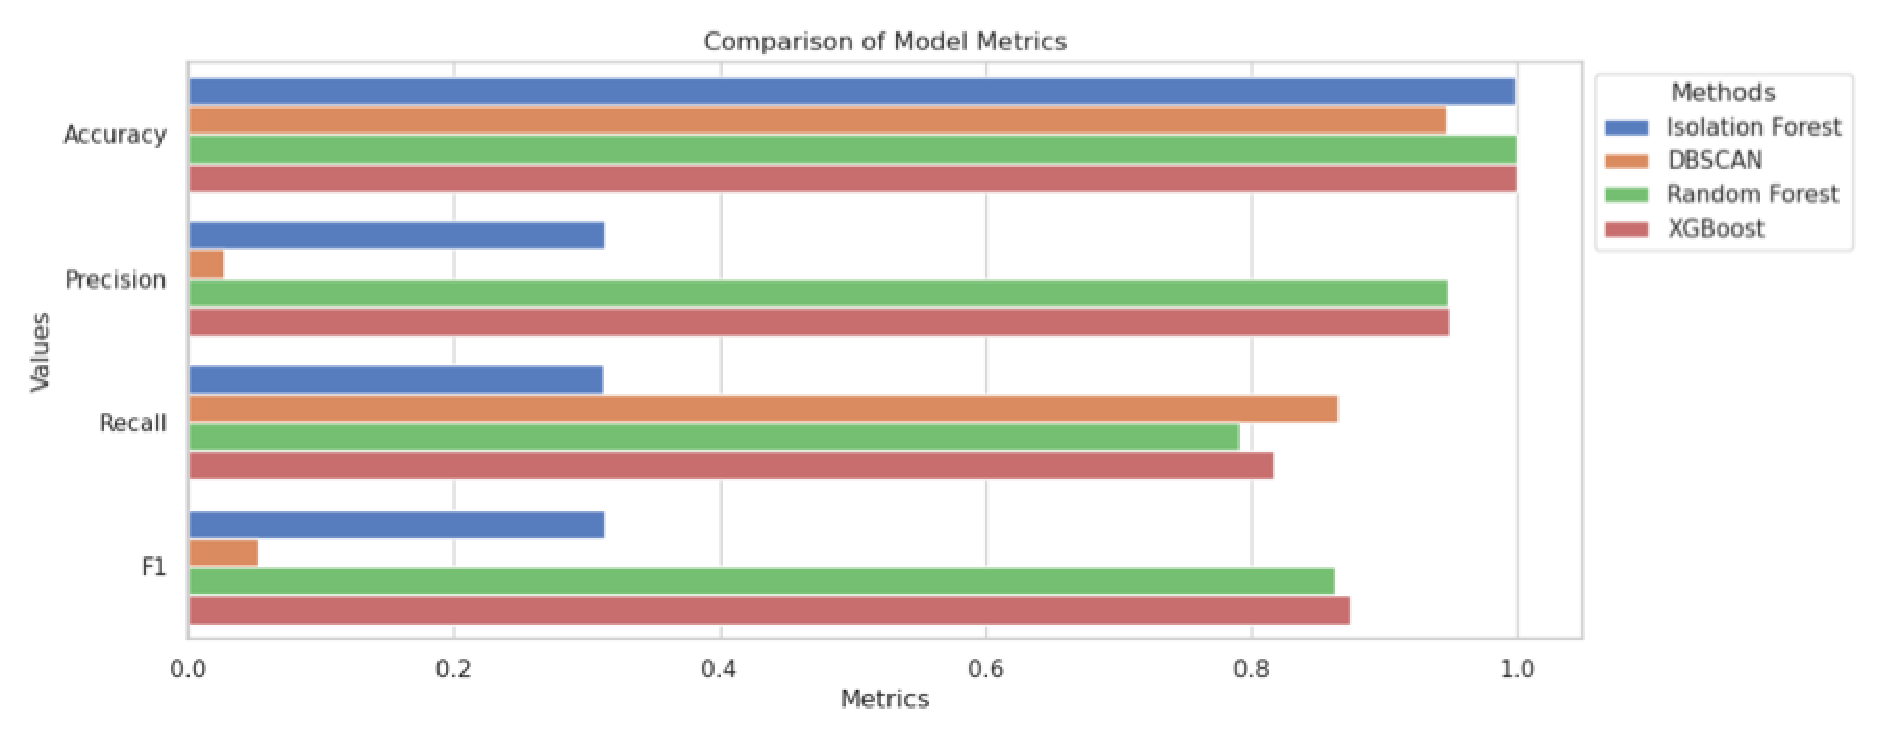
\includegraphics[scale=0.4]{result.eps}
		\caption{Comparison of Model Metrics}\label{fig:OutAspect-target}
	%  \includegraphics[width=0.5\textwidth]{figures//OutAspect_target.eps}\\

\end{figure}



\section{Conclusions} \label{sec-conclusions}
This paper compares a variety of similar models and analyzes the difference between unsupervised and supervised learning methods for anomaly detection tasks, for specific data, supervised learning methods perform better but have poorer generalizability and are prone to overfitting, and perform better for similar data, whereas unsupervised learning methods do not need to be labeled ahead of time and have good generalizability but have poorer performance and need to be tuned to the parameter.

Supervised methods are superior to unsupervised methods.The performance of decision tree related methods is related to the number of decision trees and max depth.Based on correlation analysis and feature importance analysis, identifying credit card fraud is mainly related to features V4, V10, V11, V12, V14, and V17.
	\begin{figure}[H]
	\centering
	\selectcolormodel{rgb}
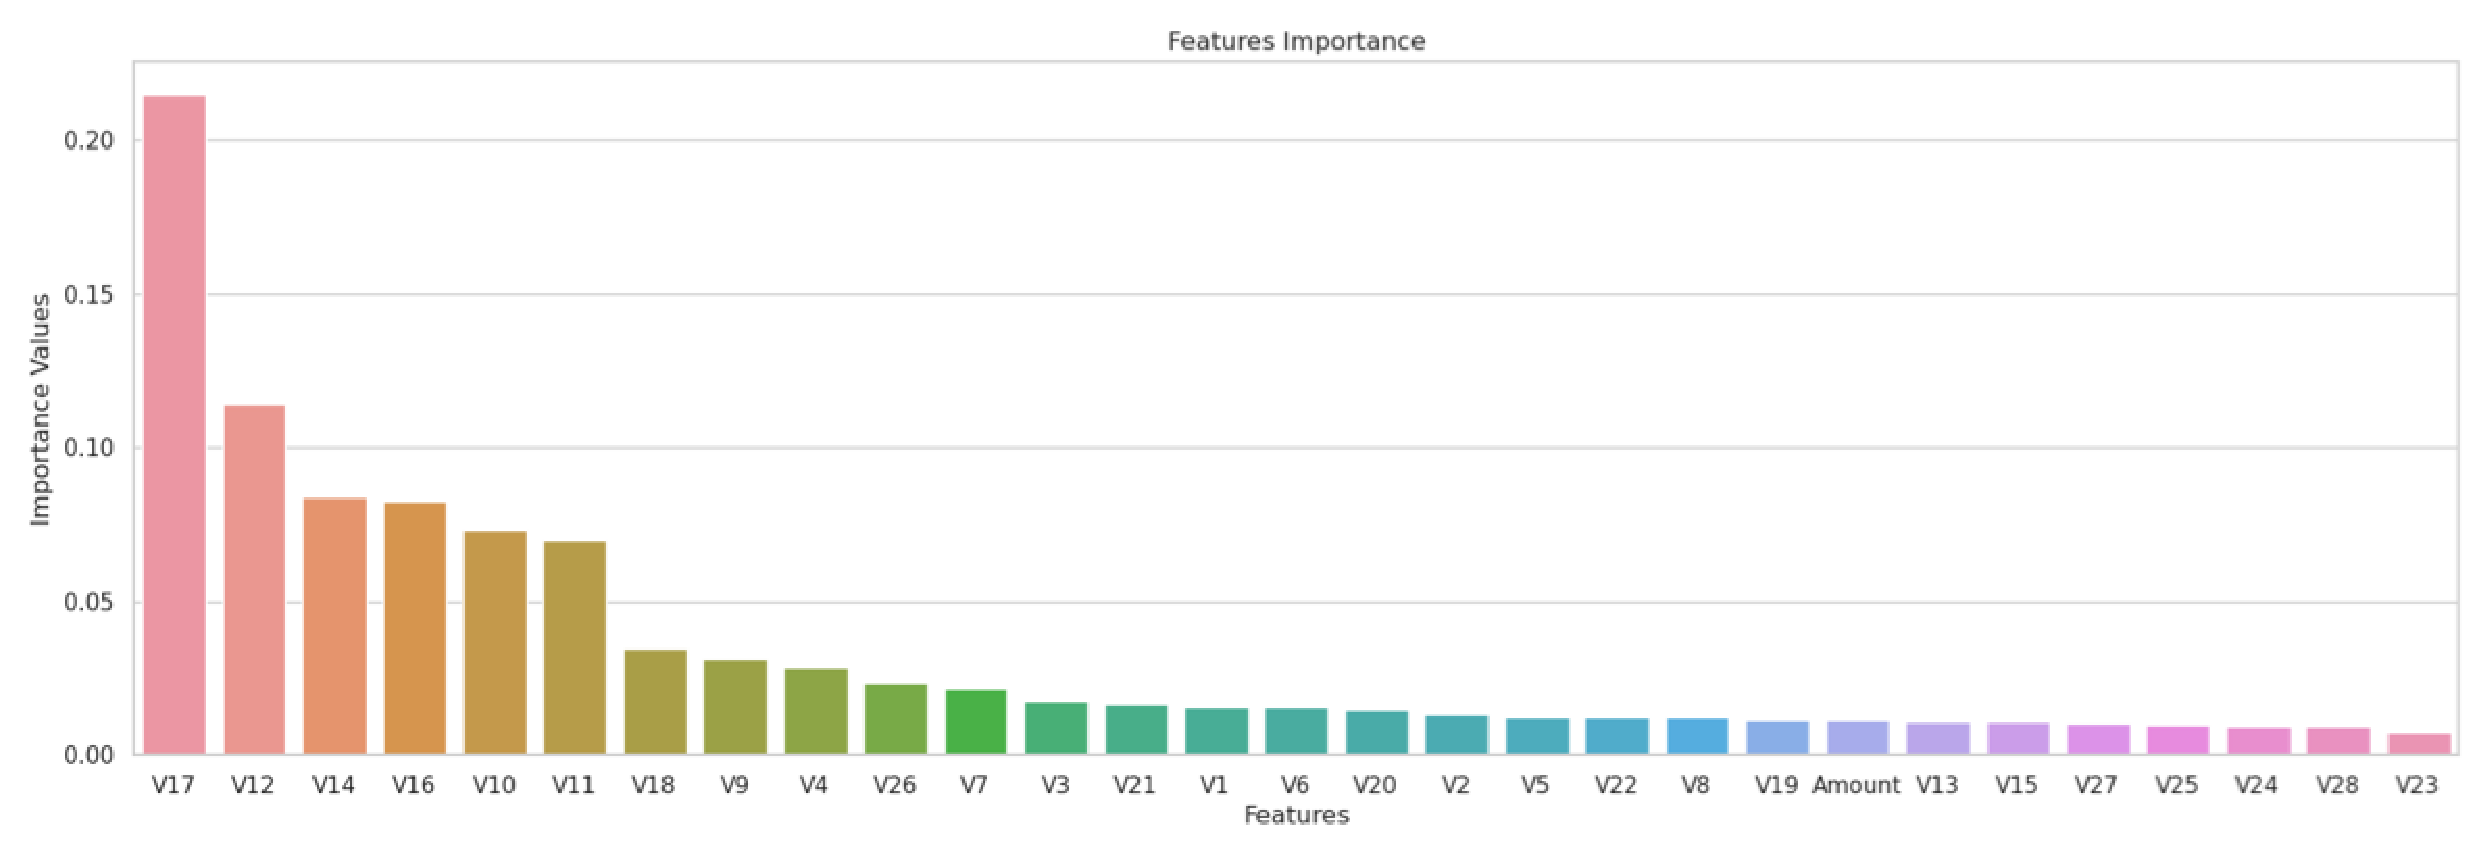
\includegraphics[scale=0.3]{fi.eps}
	%  \includegraphics[width=0.5\textwidth]{figures//OutAspect_target.eps}\\
	\caption{Feature Importance}\label{fig:OutAspect-target}
\end{figure}





